\chapter{Analyse}
\label{chap:analyse}

Ce chapitre présente l'exploration du fonctionnement des différents éléments tel que la caméra, la graveuse laser, l'écran tactile, la prise en main du bras robot \gls{ufactory} \gls{xarm6} et du logiciel \gls{aica} Studio. Il s'agit d'une étape de découverte et d'apprentissage des outils et des technologies utilisées. Cela permet également de prouver le faisabilité du projet.

\section{Prise en main du bras robot}
La prise en main du bras robot \gls{ufactory} \gls{xarm6} a été l'une des premières étapes du projet. Le but était de se familiariser avec les commandes et de comprendre les limites physiques et logicielles du robot.

\subsection{Mise en marche du robot et connexion}
Avec le manuel utilisateur fourni par Ufactory \cite{UserManual}, il a été possible de comprendre et prendre en main le robot. La première étape après la mise sous tension à été la connexion ethernet entre le contrôleur et le logiciel UFACTORY-Studio. La procédure est très simple et ne demande aucune configuration particulière.

\subsection{UFACTORY-Studio}
Le logiciel UFACTORY-Studio est utile pour configurer la position initiale du robot, les limites de mouvements, la force maximale de chaque articulation et les limites de distances à ne pas dépasser.

En plus de cela, le logiciel offre un contrôle complet sur les entrées/sorties (appelées par la suite \gls{io}), les axes, la vitesse de déplacement et l'ouverture/fermeture de la pince. Il est également possible de créer des programmes de mouvements en utilisant le langage  de programation \gls{python} ou un langage visuel propriétaire basé sur le \gls{python}. Le langage visuel reste très basique et ne permet pas de créer des programmes complexes qui sortent du cadre de la cinématique du robot.

\subsection{\gls{python} \gls{sdk}}
Pour s'affranchir des limitations du logiciel UFACTORY-Studio, il est possible d'utiliser le \gls{sdk} \gls{python} \cite{PythonSDK} fourni par \gls{ufactory}. Ce \gls{sdk} permet de contrôler le robot de manière plus avancée et de créer des programmes plus complexes. Le langage de base de contrôle du robot étant \gls{python}, il est possible d'utiliser n'importe quel \gls{IDE} \gls{python} pour développer des programmes. La documentation du \gls{sdk} étant très complète avec de nombreux exemples, la compréhension et la prise en main du SDK se sont faites rapidement. De plus, les contrôles de cinématique sont plus bas niveau ce qui offre plus de flexibilité notamment au niveau de l'accéleration, du \gls{jerk} et des opérations sur les positions.

\subsection{Entrées/sorties}
Le contrôleur du bras robot offre plusieurs types d'\gls{io}:

\definecolor{SafetyColor}{HTML}{FFDDC1}
\definecolor{PowerColor}{HTML}{C1E1FF}
\definecolor{ConfigInputColor}{HTML}{D4FFC1}
\definecolor{DigitalInputColor}{HTML}{FFD1DC}
\definecolor{ConfigOutputColor}{HTML}{E1C1FF}
\definecolor{DigitalOutputColor}{HTML}{C1FFE1}
\definecolor{RS485Color}{HTML}{FFC1E1}
\definecolor{AnalogColor}{HTML}{E1FFC1}

\begin{tcolorbox}[colframe=black, colback=SafetyColor, title=Safety]
    \textbf{Connexions :} GND | EI0 | GND | EI1 | GND | SI0 | GND | SI1
\end{tcolorbox}

\begin{tcolorbox}[colframe=black, colback=PowerColor, title=Power]
    \textbf{Connexions :} PWR | 24V-IN | GND | RI0 | NC | GND | ON | OFF
\end{tcolorbox}

\begin{tcolorbox}[colframe=black, colback=ConfigInputColor, title=Configurable Inputs]
    \textbf{Connexions :} GND | CI0 | CI1 | CI2 | CI3 | GND | CI4 | CI5 |CI6 | CI7
\end{tcolorbox}

\begin{tcolorbox}[colframe=black, colback=DigitalInputColor, title=Digital Inputs]
    \textbf{Connexions :} GND |  DI0 | DI1 | DI2 | DI3 | GND | DI4 | DI5 | DI6 | DI7
\end{tcolorbox}

\begin{tcolorbox}[colframe=black, colback=ConfigOutputColor, title=Configurable Outputs]
    \textbf{Connexions :} 24V | CO0 | CO1 | CO2 | CO3 | 24V | CO4 | CO5 | CO6 | CO7
\end{tcolorbox}

\begin{tcolorbox}[colframe=black, colback=DigitalOutputColor, title=Digital Outputs]
    \textbf{Connexions :} 24V | DO0 | DO1 | DO2 | DO3 | 24V | DO4 | DO5 | DO6 | DO7
\end{tcolorbox}

\begin{tcolorbox}[colframe=black, colback=RS485Color, title=RS485]
    \textbf{Connexions :} 24V | 24V | M\_A | M\_B | GND | L\_A | L\_B | GND
\end{tcolorbox}

\begin{tcolorbox}[colframe=black, colback=AnalogColor, title=Analog]
    \textbf{Connexions :} GND | AI0 | GND | AI1 | GND | AO0 | GND | AO1
\end{tcolorbox}

Ces \gls{io} permettent la communication avec des éléments externes.

\section{\gls{aicaS}}

\gls{aicaS} est une plateforme logicielle dédiée à l'intégration, la programmation et la supervision de robots industriels. Son principal atout réside dans son interface graphique intuitive, qui permet de concevoir des programmes complexes à l'aide de blocs fonctionnels visuels, sans nécessiter de compétences avancées en programmation.

\gls{aicaS} est un logiciel permettant d’intégrer et de programmer des robots industriels à l’aide de blocs fonctionnels visuels. Il est compatible avec plusieurs robots, dont le bras \gls{ufactory} \gls{xarm6} utilisé ici. L’utilisateur peut assembler des séquences d’actions à partir d’une bibliothèque de blocs prédéfinis (mouvements, entrées/sorties, communication, etc.), ce qui facilite la création de programmes sans avoir à écrire de code complexe.

Le logiciel repose sur \gls{ros2}, qui gère la communication entre les différents éléments du système. \gls{aicaS} masque la plupart des aspects techniques de \gls{ros2} et propose une interface simplifiée pour la gestion des tâches courantes (planification de trajectoires, synchronisation de périphériques, gestion des signaux, etc.).

Il est possible d’ajouter des blocs personnalisés en \gls{python} pour répondre à des besoins spécifiques, par exemple pour le traitement d’images ou l’automatisation de certaines tâches. Cette solution est d'ailleurs grandement utilisée dans ce travail. L’environnement propose aussi des outils de visualisation (\gls{rviz}), de simulation et de diagnostique, utiles pour le développement et la maintenance.

Malgré ses avantages, \gls{aicaS} présente certaines limites : la prise en main reste plus facile qu’avec des outils purement textuels, mais il est tout de même nécessaire de comprendre les bases de la programmation et de \gls{ros2} pour exploiter pleinement le logiciel. De plus, la configuration de certains blocs ou l’intégration de fonctionnalités avancées peuvent s’avérer complexes ou manquer de flexibilité selon les cas. Le logiciel reste tout de même un outil puissant et reçoit régulièrement des mises à jour pour améliorer ses fonctionnalités et sa stabilité.

\subsection{Installation de \gls{aicaS}}
L'installation de \gls{aicaS} est plus complexe que celle de UFACTORY-Studio. Il est nécessaire d'utiliser un système d'exploitation Linux. Le guide d'installation \cite{AICADocs} est complet et facile à suivre. Cependant, il est tout de même nécessaire d'avoir quelques connaissance de base en ligne de commandes et en gestion de systèmes Linux. L'avantage de cette installation est qu'elle permet de créer un environnement complet en incluant dans un \gls{conteneur} \gls{docker}, tous les outils nécessaire au bon fonctionnement de l'application.

\subsection{Démarrage de \gls{aicaS}}
Le démarrage de \gls{aicaS} suit la procédure strandard des applications Linux. Lorsque l'application est lancée pour la première fois, une fenêtre de configuration s'ouvre pour permettre d'entrer la clef de licence. Par la suite, l'application se lance et affiche une page de réglages pour choisir la version, les paquets à installer et les volumes partagés pour l'utilisation de fichiers.

\begin{figure}[H]
    \centering
    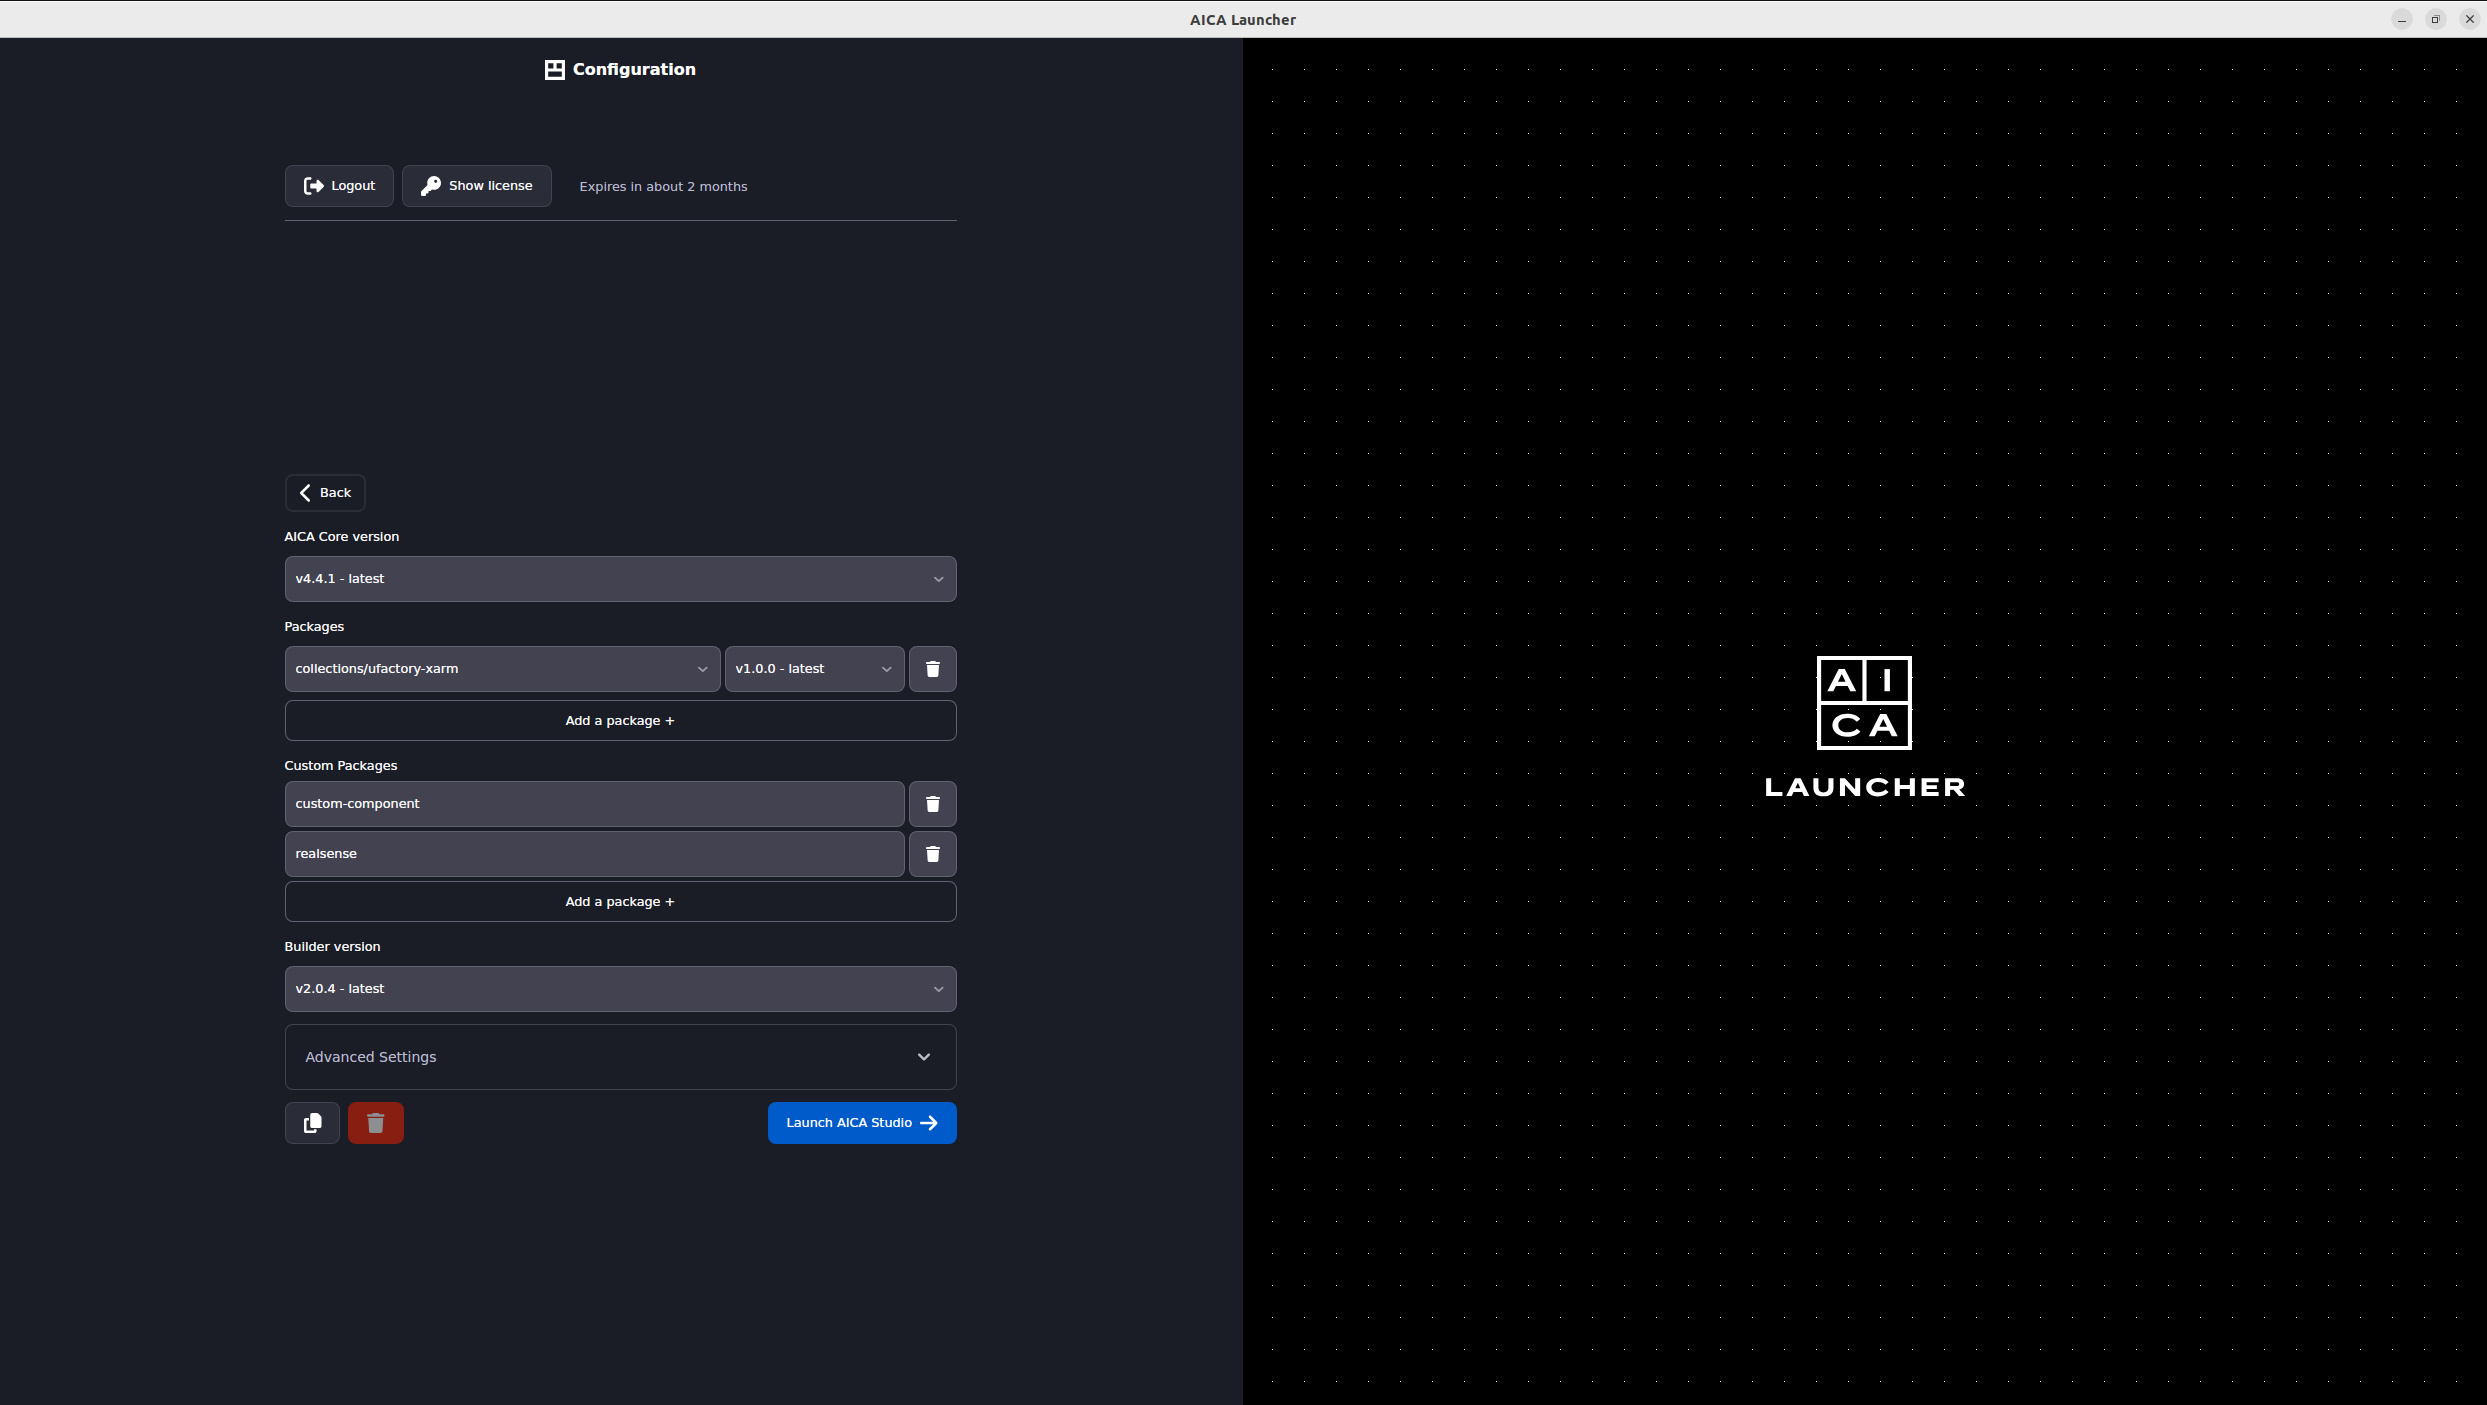
\includegraphics[width=0.8\textwidth]{assets/figures/AICA_Mainmenu.png}
    \caption{Page de démarrage de \gls{aicaS}}
    \label{fig:aica_startup}
\end{figure}

\subsection{Interface de AICA Studio}
Le logiciel est relativement intuitif et facile à prendre en main pour ce qui est de la création de programmes et la connexion des blocs fonctionnels. Cependant à l'heure actuelle, il est nécessaire de comprendre des concepts de base de la programmation (comme la syntaxe) avec \gls{ros2} pour pouvoir maitriser et utiliser les différentes possibilités offertes par le logiciel. Il est donc recommandé de parcourir les tutoriels et la documentation fournie par \gls{aica} ,ainsi que parcourir les ressources en ligne pour se familiariser avec les concepts de base de \gls{aicaS} avant de se lancer dans la création de programmes.

Il est possible de créer des programmes de deux manières différentes avec \gls{aicaS} :
\begin{itemize}
    \item En utilisant des blocs fonctionnels prédéfinis, qui permettent de créer des programmes de manière visuelle en connectant les blocs entre eux;
    \item En utilisant la fenêtre de programmation \gls{yaml}, qui permet d'avoir une vison plus detaillée du programme et de modifier les paramètres sans passer par la fenêtre de configuration des blocs.
\end{itemize}

\begin{figure}[H]
    \centering
    \begin{subfigure}{0.48\textwidth}
        \centering
        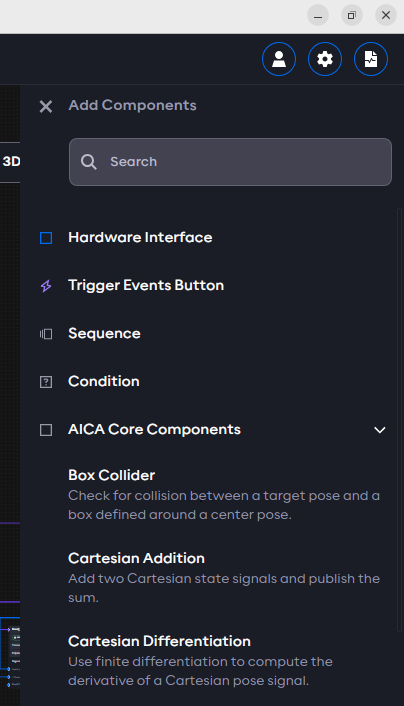
\includegraphics[width=0.95\linewidth]{assets/figures/AICA_blocs_fonct.png}
        \caption{Programmation par blocs visuels}
        \label{fig:prog_blocs_visuels}
    \end{subfigure}
    \hfill
    \begin{subfigure}{0.48\textwidth}
        \centering
        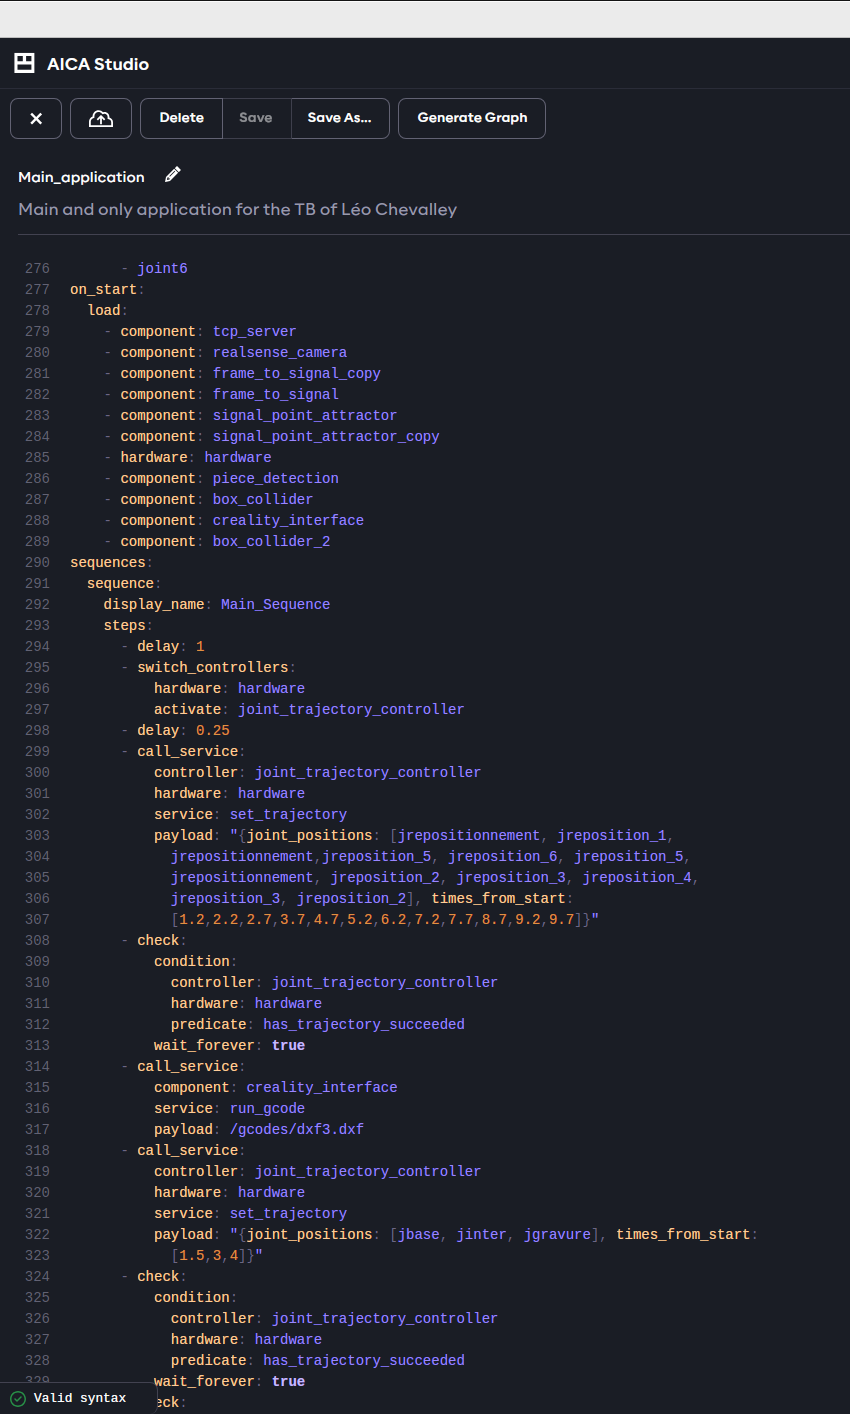
\includegraphics[width=0.95\linewidth]{assets/figures/AICA_Yaml.png}
        \caption{Programmation via \gls{yaml}}
        \label{fig:prog_yaml}
    \end{subfigure}
    \caption{Comparaison entre la programmation visuelle et la programmation \gls{yaml} dans \gls{aicaS}.}
    \label{fig:comparaison_yaml_visuel}
\end{figure}

Ces deux approches ont chacune leurs avantages et inconvénients.
D'une part la programation visuelle ne nécessite pas de connaissances particulières dans la syntaxe et la structure des langages de programmation. De plus, les liens entre les blocs sont clairs et permettent de visualiser rapidement le fonctionnement du programme. Néanmoins, la programmation visuelle ne permet pas d'avoir de vision très fine du programme. Les réglages et les paramètres des blocs doivent être ajustés individuellement dans chaque menu, ce qui rend la configuration parfois laborieuse et peu efficace lorsque de nombreux blocs sont impliqués.

Concernant la programation par le langage \gls{yaml}, elle permet d'accéder aux réglages du programme directement et de manière globale. Par contre, Il est nécessaire d'avoir de bonne bases de programmation et un bon contrôle de la syntaxe pour éviter les erreurs.

Concernant le reste de l'interface, le logiciel contient :

\begin{itemize}
    \item Une barre de menu, qui permet d'accéder à la documentation, aux contrôles \gls{hardware} et à la page programmation par blocs (voir a);
    \item Un onglet réglages qui permet de redémarrer l'application, accéder au terminal et démarrer à \gls{rviz} (voir b);
    \item Un bouton pour accéder aux \gls{logs} de l'application (voir c);
    \item Des boutons d'actions pour le démarrage, l'arrêt et le rechargement du programme (voir d).
\end{itemize}

\begin{figure}[H]
    \centering
    \begin{tabular}{cc}
        \begin{subfigure}{0.45\textwidth}
            \centering
            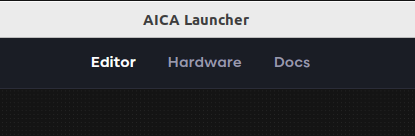
\includegraphics[width=0.9\linewidth]{assets/figures/AICA_barre_haute.png}
            \caption{Barre de menu}
            \label{fig:aica_barre_menu}
        \end{subfigure} &
        \begin{subfigure}{0.45\textwidth}
            \centering
            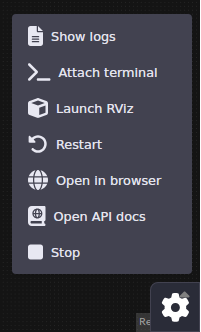
\includegraphics[width=0.9\linewidth]{assets/figures/AICA_rviz.png}
            \caption{Onglet réglages}
            \label{fig:aica_rviz}
        \end{subfigure}        \\
        \addlinespace[0.5em]
        \begin{subfigure}{0.45\textwidth}
            \centering
            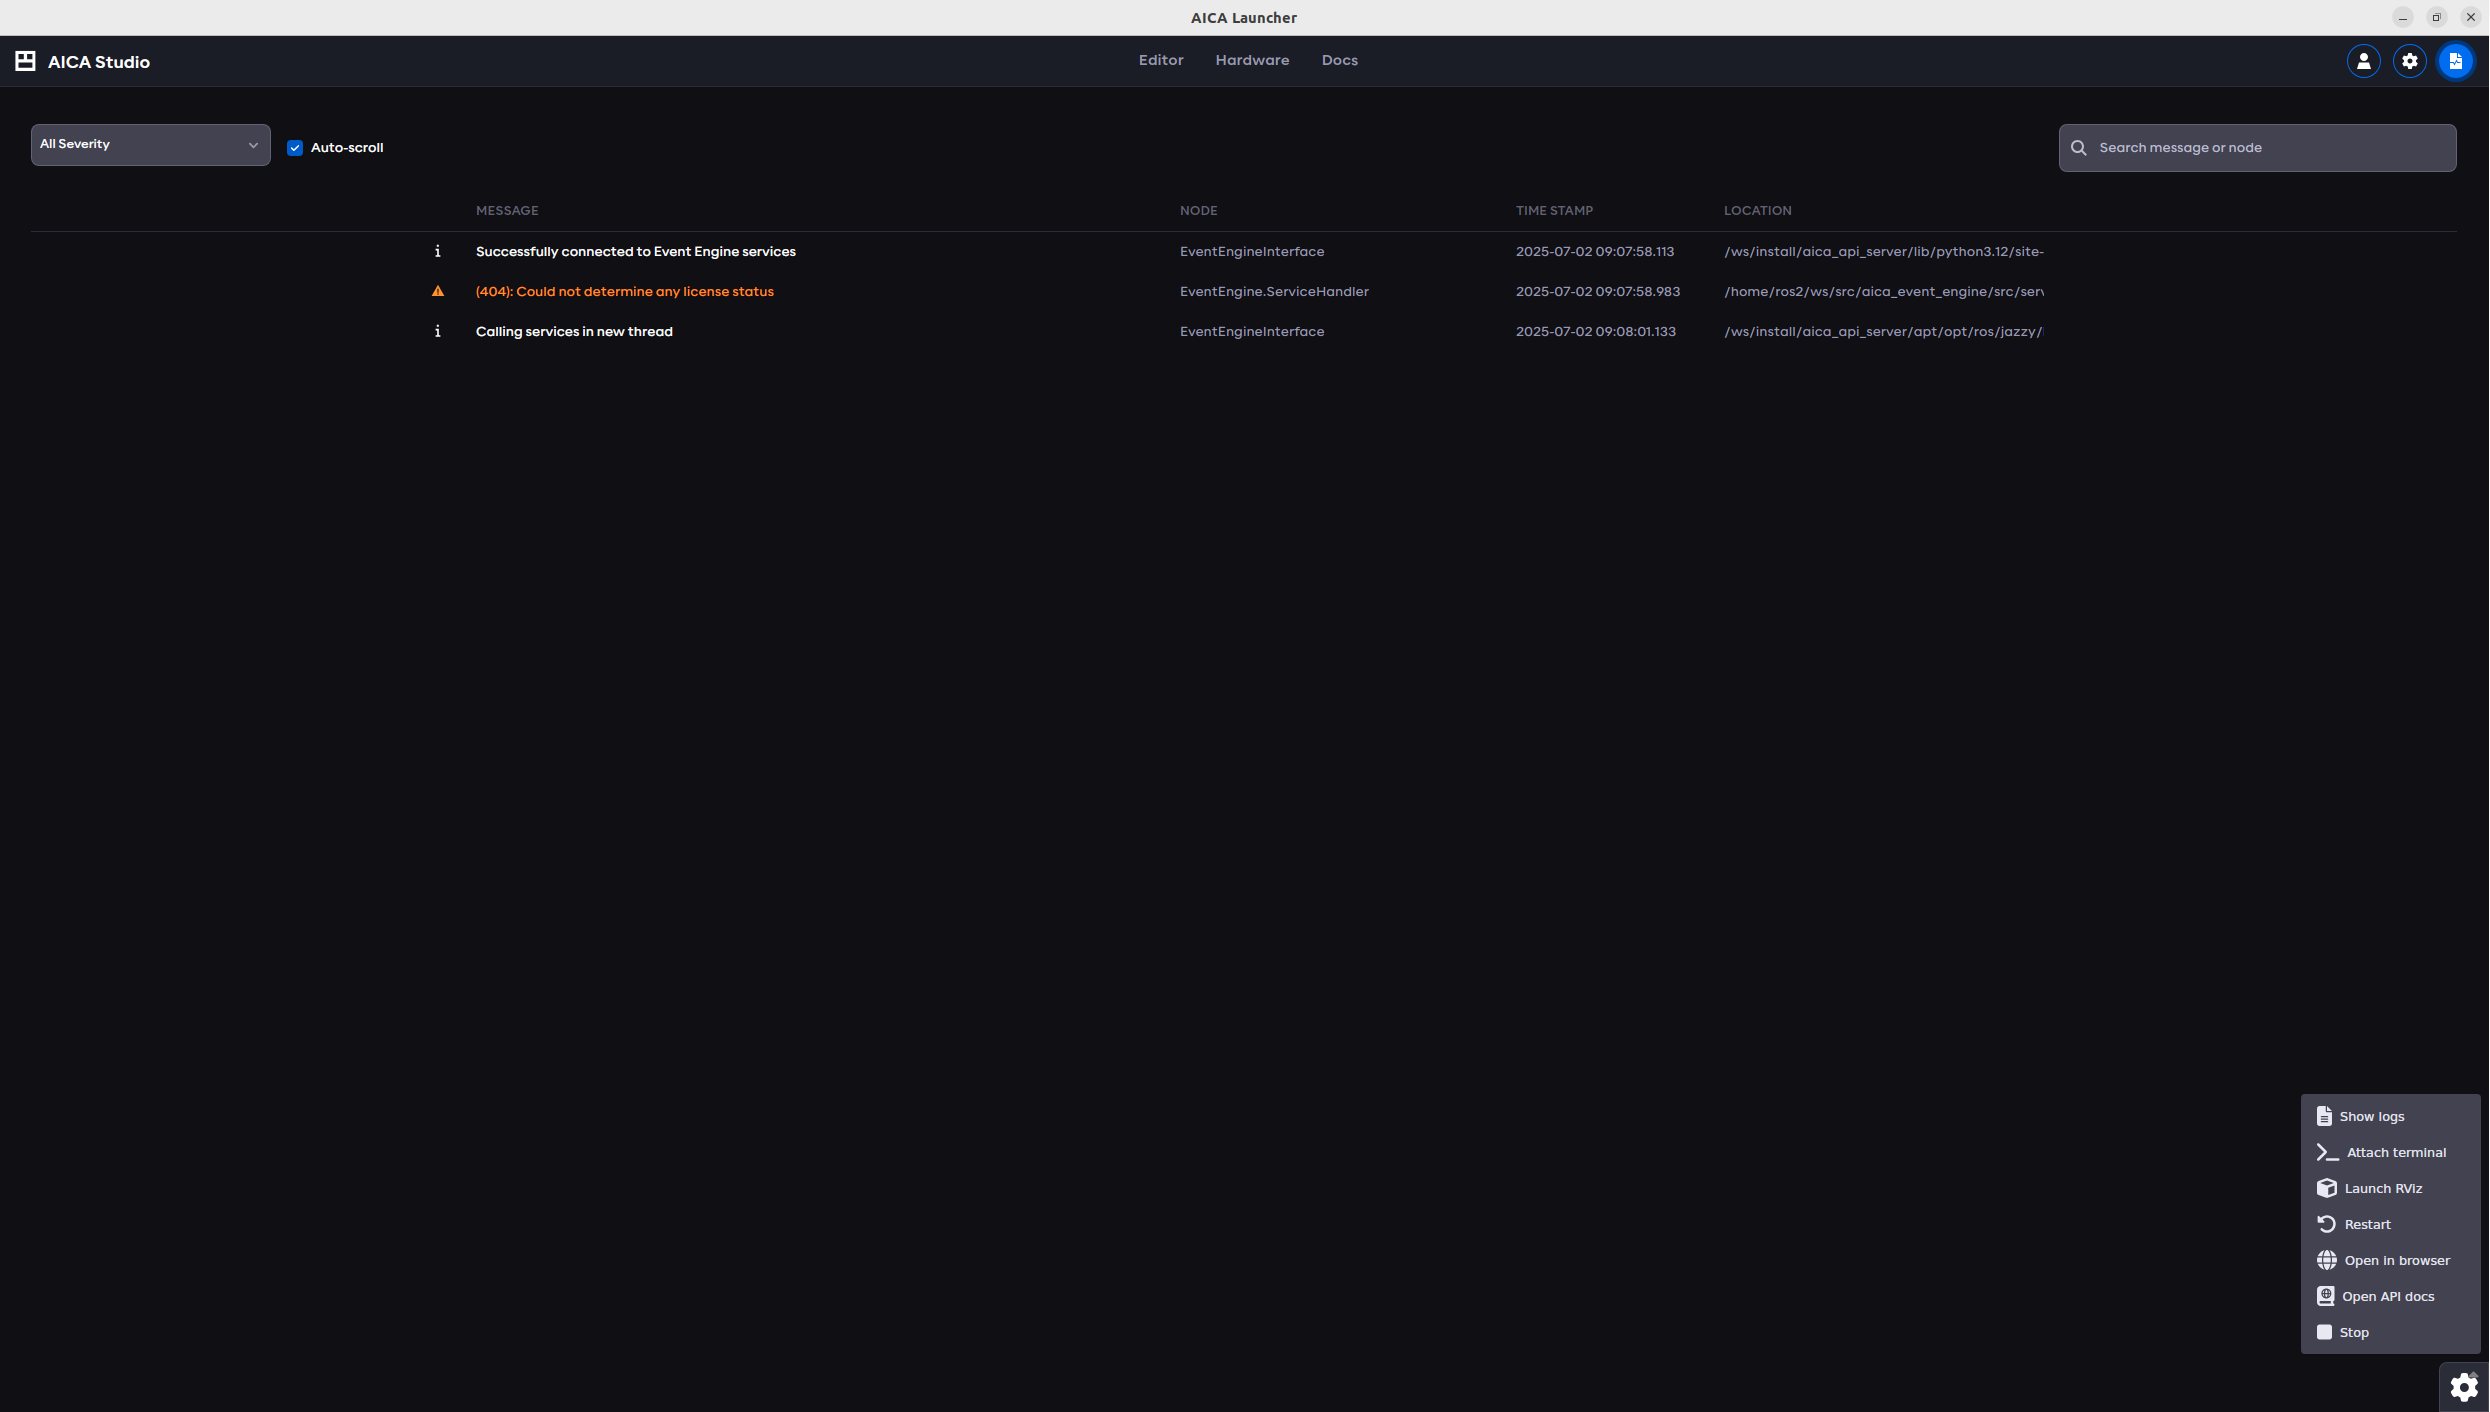
\includegraphics[width=0.9\linewidth]{assets/figures/AICA_logs.png}
            \caption{Bouton logs}
            \label{fig:aica_logs}
        \end{subfigure}        &
        \begin{subfigure}{0.45\textwidth}
            \centering
            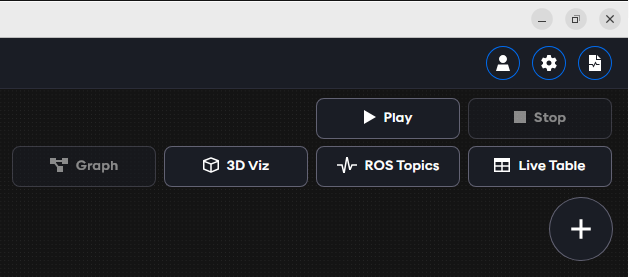
\includegraphics[width=0.9\linewidth]{assets/figures/AICA_play_pause.png}
            \caption{Boutons d'action}
            \label{fig:aica_play_pause}
        \end{subfigure}
    \end{tabular}
    \caption{Principaux éléments de l'interface de \gls{aicaS}.}
    \label{fig:aica_interface_elements}
\end{figure}

Ces éléments permettent de naviguer facilement dans l'application et d'accéder aux différentes fonctionnalités. L'interface est conçue pour être intuitive et facile à utiliser. Malgré les limitations actuelles du logiciel et la nécessité de comprendre les concepts de base de \gls{ros2} ainsi que les premières versions de \gls{aicaS}, l'interface utilisateur est à présent agréable à utiliser.

\section{Analyse de la caméra Intel RealSense D435}
La caméra Intel RealSense D435 joue un rôle central dans la détection automatique des pièces à graver. Son capteur de profondeur permet de localiser précisément les objets dans l’espace de travail.
\subsection{Principes de fonctionnement}
La caméra utilise la technologie de stéréovision pour générer un nuage de points 3D. Cela permet d’obtenir la position et l’orientation des pièces avec une grande précision.
\subsection{Intégration dans le système}
La caméra est montée sur la maquette de façon à couvrir toute la zone de prise. Les données sont traitées en temps réel par un bloc fonctionnel dans \gls{aicaS}.
\subsection{Limites et contraintes}
La qualité de la détection dépend fortement de l’éclairage et de la couleur des pièces. Des tests ont montré que certaines couleurs ou reflets peuvent perturber l’algorithme.

\section{Analyse de la graveuse laser Creality Falcon}
La graveuse laser Creality Falcon est utilisée pour réaliser la gravure sur les pièces détectées.
\subsection{Caractéristiques techniques}
La machine offre une bonne précision et une puissance adaptée à la gravure sur différents matériaux. Elle est compatible avec les fichiers \gls{gcode} générés automatiquement.
\subsection{Intégration et contrôle}
La graveuse est pilotée via un bloc fonctionnel dans \gls{aicaS}, qui reçoit les instructions de gravure après la détection et le positionnement de la pièce.
\subsection{Limites et points d’attention}
La synchronisation avec le robot est essentielle pour éviter les erreurs de gravure. La machine doit être correctement positionnée et sécurisée pour garantir la qualité et la sécurité du processus.

\section{Analyse de l’écran tactile ED-101}
L’écran tactile ED-HMI3010-101C (ED-101) permet à l’utilisateur de dessiner le motif à graver et de l'envoyer au système.
\subsection{Interface utilisateur}
L’application développée en \gls{python} (Tkinter) offre une interface intuitive pour dessiner, sélectionner des formes et envoyer le fichier \gls{dxf} au système.
\subsection{Communication et intégration}
L’écran communique avec le PC principal via le réseau, et le fichier \gls{dxf} est transmis au bloc fonctionnel de la graveuse laser.


\section{Limites}
Bien que la station de gravure laser intelligente réponde aux besoins initiaux du projet, certaines limites ont été identifiées:
\begin{itemize}
    \item \textbf{Dépendance logicielle} : Le système repose sur un logiciel propriétaire (\gls{aicaS}) qui peut évoluer ou devenir obsolète. Il est également nécessaire d'avoir une clef de licence pour utiliser le logiciel, ce qui peut s'avérer couteux à long terme.
    \item \textbf{Sécurité} : Malgré les mesures prévues, la sécurité en contexte public dépend fortement de la vigilance de l'opérateur.
    \item \textbf{Flexibilité des scénarios} : Le système est optimisé pour la démonstration, mais moins adapté à une production industrielle ou à des pièces très variées.
\end{itemize}

Cette réflexion permet d'ouvrir le projet à de futures évolutions et d'envisager des applications plus larges ou plus exigeantes.



